\documentclass[12pt]{article}

% -- fonts (Times Roman via TeX Gyre Termes) --
\usepackage[T1]{fontenc}
\usepackage{lmodern}
\usepackage{tgtermes}

% -- layout --
\usepackage[margin=1in]{geometry}
\usepackage{setspace}
\doublespacing

% -- line numbers --
\usepackage{lineno}
\linenumbers

% -- math --
\usepackage{amsmath}

% -- tables --
\usepackage{booktabs}

% -- figures --
\usepackage{graphicx}
% author-year citations with round brackets, as required by the journal
\usepackage[round,authoryear]{natbib}
\bibliographystyle{plainnat}

% -- hyperlinks (no colored links) --
\usepackage[colorlinks=false,hidelinks]{hyperref}

% -- breakable file paths: \path{} allows line breaks inside long
%    directory/file names, which \texttt{} cannot do --
\usepackage{url}
\urlstyle{tt}
\def\UrlBreaks{\do\/\do\_\do\-\do\.}

% -- PLOS requires "Fig" not "Figure" --
\renewcommand{\figurename}{Fig}

% ============================================================
% TITLE AND AUTHOR
% ============================================================

\title{Code Geometry, Enforcement Activation, and Exit Closure in Codified Moral Systems: An Agent-Based Model}

\author{}

\date{}

\newcommand{\affiliation}{}

\date{}

\begin{document}

\maketitle
%\noindent\affiliation
\vspace{1em}

% ============================================================
% ABSTRACT
% ============================================================

\begin{abstract}
Why do some codified moral systems sustain active enforcement while others also retain members under durable control? This paper separates two structural dimensions in an agent-based model: activation of an enforcement apparatus and members' capacity to exit. Enforcement activation follows a joint frontier in code observability and enforcement reward. With exit open, enforcement activates in many parameter cells but capture occurs in 0 of 1,890 runs. Imposed exit closure raises capture monotonically, yet cannot produce capture in a low-observability, low-reward cell where enforcement does not activate. A privilege ablation further shows that roughly 84 percent of top-five-percent punishment concentration is manufactured by institutional advantages assigned to the enforcement cadre. A specification check establishes that making outside-option closure a function of enforcer share makes closure a function of the enforcement activity it is meant to explain. Because closure enters the exit computation directly, capture then follows by construction rather than from agent behaviour. Exit capacity is therefore modeled as an independent structural input. The model identifies distinct conditions for activation, retention, and concentration.
\end{abstract}
\vspace{1em}\noindent\textbf{Keywords:} agent-based modeling; institutional design; norm enforcement; organizational capture; path dependence; religious organizations

\newpage

% ============================================================
% 1. INTRODUCTION
% ============================================================

\section{Introduction}

Why are strict religious groups often unusually cohesive and durable? The canonical answer begins with religious organizations as clubs that produce collective goods. In Iannaccone's account, apparently wasteful demands can make these clubs stronger: costly requirements involving dress, diet, ritual, time, and money screen out people whose low commitment would otherwise permit them to free-ride on the sacrifices of others \citep{iannaccone1988,iannaccone1992,iannaccone1994}. Those who remain redirect resources away from competing activities and toward the group, increasing both the average commitment of members and the value of membership itself. Strictness, on this view, is not organizational pathology but a solution to adverse selection and weak participation. This club-goods framework has become the dominant economic explanation of religious strictness, as reviews of the economics of religion emphasize \citep{iyer2016,carvalho2019}. It has also generated an unusually broad family of applications. Sacrifice and nontransferable religious capital help explain ultra-Orthodox Jewish education and fertility \citep{berman2000}; monitoring institutions can sustain religious production \citep{mcbride2007}; costly signals can resolve commitment problems in religious militancy \citep{bermanlaitin2008}; and veiling can operate as a commitment device that changes social interaction and marriage-market incentives \citep{carvalho2013}. Across these applications, costly observances select committed participants and align their investments with the group.

Yet the same arrangements have another face. Mechanisms that screen at entry typically also raise the cost of exit after entry. A social network concentrated inside the group is valuable to a committed member, but it is also difficult to replace after departure. An identity made inseparable from membership can deepen solidarity, but it can also make departure psychologically and socially disorganizing. Distinctive dress, diet, language, schooling, and ritual can certify commitment among insiders while isolating members from outsiders who might provide employment, friendship, marriage, or recognition. Screening and exit foreclosure are therefore the same social structure described from opposite directions. Looking inward from the organizational boundary, strictness selects and coordinates participants; looking outward from the position of a member considering departure, it degrades alternatives and makes separation costly. Case scholarship often recognizes both processes at once without analytically separating them. An analysis of the Skoptsy sect, for example, argues that high entry costs screened for devoted individuals while high exit costs reduced the viable alternatives for living outside the sect [VERIFY: citation key for the Skoptsy sect analysis]. The two mechanisms can coexist, but coexistence does not establish which one accounts for durability.

That ambiguity is now a live theoretical problem rather than a terminological distinction. \citet{bok2025} observes that research on religious exit has concentrated mainly on who leaves, why they leave, and what follows, while the forms and roles of exit costs have received comparatively little systematic theorization. The systematic theorization of the exit-cost side is therefore recent relative to the mature literature on the determinants and consequences of exit. The field has a mature screening account and a newly articulated exit-cost problem, but no design that can adjudicate their relative causal force. The identification problem is plain. In observational data, screening and exit foreclosure arrive bundled together. Any strict group that persists has already selected some people willing to bear its demands and has also organized relationships, identities, and opportunities in ways that make leaving consequential. Comparing strict and lenient groups cannot recover the separate contribution of either process, because the strictness that filters entrants also transforms the outside option of those who stay. Nor can studying former members solve the problem by itself: observed leavers are selected on having overcome the very costs whose preventive effect is at issue. Without independent variation, evidence consistent with successful screening is also consistent with blocked exit.

Agent-based simulation supplies the missing instrument because it permits the two structures to be varied as distinct inputs while measuring any coupling between their effects. An experimental design can hold the observability and rewards that support enforcement constant while changing members' capacity to leave, or hold exit conditions constant while changing whether an enforcement apparatus can activate. No observational design can cleanly impose either intervention on otherwise equivalent religious communities. The strategy follows an established computational-religion program associated with Shults and Wildman [VERIFY: publication year and citation key for Shults and Wildman], formal arguments for bringing simulation into the study of religion \citep{wildmansosis2011}, computational work linking cognition, culture, and social dynamics \citep{gorelemosshultswildman2018}, and agent-based analysis in the economics of religion \citep{iannacconemakowsky2007}. Simulation here is therefore not a substitute for historical or ethnographic evidence. It is a method for identifying structural effects that those forms of evidence necessarily observe in combination.

This paper distinguishes two structural dimensions that are largely separable, but coupled at the frontier margin: whether an enforcement apparatus activates, and whether members can leave. The quantitative caveat to this separation is reported in the results. Three findings result. First, activation follows a joint threshold in code observability and the reward for enforcement. Neither condition is sufficient alone. Across a 63-cell grid crossing nine observability levels with seven reward levels, enforcement appears along a frontier defined jointly by both parameters rather than along either axis independently. Second, exit closure is necessary but not sufficient for capture. In the exogenous closure experiment, the capture rate rises monotonically from 0 at fully open exit to 0.889 at the maximum imposed closure. Yet the low-observability, low-reward cell remains at zero capture at every closure level, including the maximum. Closing exit can retain an apparatus that activates, but it cannot create one where enforcement lacks both legibility and reward. Third, the concentration of punishment that appears to mark enforcement-dominant regimes is largely manufactured by institutional privilege. In the floor-versus-ceiling ablation, the top 5 percent of active agents issue 0.091 of punishments without the privilege bundle and 0.580 with it. Relative to the ceiling, 0.843, or roughly 84 percent, of top-5-percent concentration is privilege-manufactured. The floor Gini is 0.240, compared with 0.028 under a same-volume random-allocation null. These results distinguish the conditions that form enforcement, retain its subjects, and concentrate coercive activity. As a specification check, an outside-option closure rule driven by enforcer share makes closure a function of the enforcement activity it is meant to explain. Because closure enters the exit computation directly, capture then follows by construction rather than from agent behaviour. Exit capacity is therefore treated as an independent structural input; decoupled closure produces 0 capture in 4,050 runs at each tested coupling strength.

The concentration result also qualifies a prominent interpretation in the punishment literature. The costly-punishment tradition asks how sanctioning can arise through decentralized interaction even when punishers bear private costs. Experimental and evolutionary models show how punishment can sustain cooperation and how sanctioning behavior can spread or persist under specified population and institutional conditions \citep{fehrgachter2000,boydgintisbowles2010,hauertetal2007}. From that perspective, a skewed distribution of punishment may look like an emergent product of heterogeneous strategies, repeated interaction, or selection among decentralized actors. The ablation suggests a different interpretation for delegated architectures. When one role enjoys exclusive or strongly asymmetric authority, lower costs and risks, and material reinforcement, concentrated sanctioning is substantially built into the opportunity structure before interaction generates any further inequality. This is not a general claim that punishment concentration never emerges from decentralized dynamics. It is a bounded contrast: in models with an institutionally privileged enforcement role, observed concentration cannot be treated as evidence of decentralized emergence without first removing or measuring the privileges that allocate coercive opportunities.

The mechanism is content-neutral. It is defined over structural properties: how observable a code's requirements are, what rewards attach to enforcing them, whether sanctioning authority is delegated asymmetrically, and how costly it is for a member to leave. Nothing in this definition depends on the truth, theology, or substantive moral content of a doctrine. The same logic can apply to any organization that codifies conduct and attaches status to compliance, including political movements, residential communities, firms, schools, or ideological associations. Religious regimes provide the empirical terrain because they offer the longest and richest documented record of codified conduct, costly membership, delegated moral authority, and contested exit. They also make the duality especially visible, since practices experienced as identity, discipline, and mutual commitment by some members may function as barriers to outside life for others. The paper makes no claim that codified belief tends toward coercion. Its claim is conditional and structural: where observable rules, enforcement rewards, delegated privileges, and constrained exit combine, they generate dynamics that cannot be inferred from doctrine alone.

The remainder of the paper develops the argument in four steps. The next section connects screening, exit costs, and costly punishment and derives the hypotheses. The methods section specifies the agent-based design and the independent interventions on activation, exit, and privilege. The results section presents the activation frontier, exit-closure dose-response, and privilege ablation. The conclusion states the empirical implications, limits, and tests that follow from separating selection into a group from members' capacity to leave it.

\section{Literature Positioning}

\subsection{Enforcement and strictness in the rational-choice tradition}

The dominant formal framework for understanding why high-cost religious groups persist and grow is the club-goods model developed by \citet{iannaccone1992,iannaccone1994}. In this framework, costly behavioral demands (dietary restrictions, dress codes, tithing, time-intensive rituals) function as screening mechanisms that exclude free-riders, raising the average quality of participation and the value of club goods (mutual aid, social capital, communal identity). Strictness is the price of admission; groups that charge higher prices attract more committed members and outcompete lenient groups in cohesion and mobilization.

This framework captures an important mechanism, and the empirical pattern it explains (that strict denominations grow while lenient ones decline) is robust. But it leaves three questions unanswered that are central to the phenomenon of enforcement-dominant dynamics. First, enforcement in the club model operates through screening (an ex ante mechanism): costly demands filter the population before entry. The model does not address ex post enforcement: the active policing, sanctioning, and punishment of members who have already joined. The transition from ``strict requirements attract committed members'' to ``enforcement specialists police the community'' is not formalized.

Second, the club model does not produce a structural distinction between moderate strictness (functional screening) and enforcement dominance (coercive control by a specialized minority). These are treated as points on a continuum rather than as qualitatively different regimes. \citet{iannaccone1994} acknowledged that excessive strictness can backfire: ``a church reaches [the tipping] point when it fails to offer acceptable substitutes for everything it has asked its members to give up,'' but the tipping point is not modeled as a regime transition. Third, the club model assumes voluntary participation. Members choose the strict bundle; those who dislike it leave. This assumption is reasonable for denominational choice in pluralistic religious markets but fails in contexts where exit is blocked, where apostasy carries legal penalties, kinship networks are wholly internal, or economic livelihood depends on community membership.

\citet{berman2000} extended the club framework to ultra-Orthodox Jewish communities, where yeshiva attendance creates non-transferable religious human capital that functions as a powerful exit cost. \citet{berman2008} applied similar logic to terrorist organizations, where sacrifice requirements solve principal-agent problems in covert operations. \citet{carvalho2013} formalized veiling as a commitment mechanism with implicit reputational costs for non-compliance. These extensions move closer to the dynamics of enforcement (Berman's religious capital is the strongest existing formalization of exit cost as a lock-in device), but in the models cited here, sanctioning is costly to the sanctioner and no institutional payoff accrues to enforcement. The gap is consistent: the club tradition explains why strict groups can be stable but does not explain how enforcement authority concentrates in a minority or how enforcement regimes become self-reinforcing.

\subsection{Punishment, monitoring, and the observability problem}

A parallel literature in evolutionary game theory addresses the conditions under which punishment can stabilize cooperation. \citet{boyd2003} demonstrated that altruistic punishment can evolve in large groups because punishment costs decrease as punishers become common. \citet{fehr2000,fehr2002} provided experimental evidence that costly punishment sustains cooperation and that cooperation collapses when punishment is unavailable. \citet{axelrod1986} showed that metanorms (punishing those who fail to punish) can stabilize norm enforcement through second-order sanctioning.

These results establish that enforcement equilibria are achievable under general conditions. But a structural feature unites these models: punishment is treated as a cost to the enforcer. Punishment is altruistic; it benefits the group at the expense of the individual punisher. This is a reasonable assumption for many settings, but it does not describe the dynamics of institutionalized enforcement in codified belief systems, where enforcers routinely gain status, institutional access, and material rewards for policing. Clerical promotion contingent on orthodoxy enforcement, social prestige for public correction of deviants, and institutional budgets tied to enforcement activity all represent positive payoffs to sanctioners. When enforcement is profitable rather than costly, the dynamics change qualitatively: enforcement becomes self-sustaining not because punishers are altruistic but because the enforcement niche is structurally rewarding.

The closest formal predecessor to this dynamic is the Emperor's Dilemma of \citet{centola2005}, an agent-based model where cascades of support for unpopular norms emerge when enforcement is observable and enforcers gain status. A small minority of ``true believers'' can induce majority compliance through self-reinforcing enforcement cascades. This model captures the core intuition (that enforcement can spread as a social strategy even without genuine belief), but it treats compliance as binary, does not model exit, and does not introduce institutional delegation or compounding enforcement capacity. The cascade operates through decentralized peer pressure rather than through a specialized enforcement apparatus.

A second structural limitation of the punishment literature is the treatment of observability. Punishment requires that defection (or noncompliance) be observable. This observation-dependence is implicit in nearly all punishment models but is rarely formalized as a variable property of the system being enforced. The degree to which a moral code renders compliance observable is not a constant; it is a design feature of the code itself. A code that demands observable acts (attend Friday prayers, wear prescribed clothing, observe dietary restrictions publicly) generates fundamentally different enforcement dynamics than a code that demands internal states (reduce anger, cultivate compassion, attain non-attachment). \citet{scott1998} developed this insight at length for state governance (standardization and simplification render populations legible to administrative control), but no formal model has applied Scott's legibility concept to belief enforcement. This gap is the origin of our $\sigma$ parameter.

\subsection{Exit, voice, and the regime problem}

\citet{hirschman1970} provides the canonical framework for organizational responses to decline in \textit{Exit, Voice, and Loyalty}: members can leave (exit), attempt reform (voice), or remain despite dissatisfaction (loyalty). Hirschman noted that religions explicitly position themselves as unsubstitutable, thereby raising loyalty and suppressing both exit and voice. The framework is structurally binary (exit or voice, modulated by loyalty) and does not distinguish between the qualitatively different outcomes that exit cost variation produces.

When exit is cheap and enforcement escalates, the expected outcome is fragmentation: dissatisfied members leave, the population contracts, and the enforcement apparatus loses targets. When exit is expensive and enforcement escalates, the expected outcome is very different: dissatisfied members are trapped, dissent is internalized, and enforcement can stabilize without corrective feedback from departures. These are not points on a continuum; they are distinct dynamical regimes with different attractor structures.

The theory of preference falsification developed by \citet{kuran1995} comes closest to formalizing this distinction. Citizens publicly express preferences differing from private beliefs under social pressure, producing ``collective conservatism'' (stable falsification) or ``revolutionary cascades'' (sudden dissolution when the falsification threshold breaks). Kuran discussed religious preference falsification explicitly (crypto-Judaism under the Inquisition, Shia taqiyya) and his two-regime structure maps partially onto the collapse and mixed-enforcement regimes in our framework. However, Kuran does not formalize hierarchical capture as a distinct stable equilibrium. For him, all falsification equilibria are potentially unstable, subject to revolutionary cascade. The possibility that an enforcement-dominant minority can stabilize the system indefinitely through institutional delegation and compounding enforcement capital, preventing cascade even when private dissent is near-universal, is outside his framework.

The leaving-religion literature \citep{bromley1998,cragun2011,streib2009} provides extensive empirical documentation of exit costs and their consequences, but this scholarship is primarily descriptive and case-based. It does not formalize how exit cost interacts with enforcement parameters to generate distinct regime types. Agent-based models of secularization \citep{gelfand2011,norenzayan2013} model affiliation and disaffiliation dynamics but typically drive these through existential security or cognitive variables rather than enforcement geometry.

\subsection{Delegation, monopoly, and the missing mechanism of minority capture}

The theoretical gap that motivates this paper sits at the intersection of three well-developed literatures that have not been formally integrated.

State-formation theory provides the vocabulary of coercive monopoly. \citet{weber1946} defined the state by its successful claim to monopoly over legitimate force. \citet{tilly1985} described state-making as organized coercion with a ratcheting dynamic: war requires taxation, taxation requires administrative capacity, administrative capacity enables more war. \citet{mann1986} distinguished despotic power (command) from infrastructural power (the capacity to penetrate society with rules and monitoring). These frameworks describe compounding coercive capacity at the macro-political level but have rarely been applied to the internal governance of belief systems.

New institutionalism provides the theory of enforcement equilibria and path dependence. \citet{north1990} defined institutions as formal and informal constraints plus enforcement characteristics, and noted that ``formal rules are created to serve the interests of those with the bargaining power to create new rules'': minority capture by institutional design. \citet{greif2006} analyzed the transition from distributed to specialized enforcement in merchant communities. \citet{greif2016} observed that ``the fact that such an agent has been asked to legitimize a ruler is a source of additional power to such agents,'' a description of compounding enforcement capital that remains unformal. \citet{pierson2000} formalized path dependence as an increasing-returns dynamic where early institutional advantages compound over time.

Political economy of religion provides case studies of enforcement delegation. \citet{rubin2017} analyzed religious authorities as ``legitimizing agents'' who sit at the political bargaining table; Ottoman ulama monopolized religious scholarship and commercial law interpretation for centuries. \citet{cook2000} traced the Islamic hisbah doctrine from individual Muslim obligation to institutional enforcement apparatus. \citet{given1997} documented how the medieval Inquisition accumulated records, informers, and procedural knowledge that compounded its enforcement capability across decades. \citet{kelly1989} described the transition from personal inquisitorial authority to institutional jurisdiction, the shift from distributed to delegated enforcement.

Each of these literatures contains ingredients of the mechanism we formalize: coercive monopoly, enforcement delegation, compounding capacity, path dependence. But they have not been combined into a unified micro-level model that derives enforcement regimes from the interaction of code structure and institutional design. Evolutionary game theory has partially filled this gap through the distinction between peer punishment and pool punishment \citep{hilbe2014,sigmund2010}, showing that delegated institutional punishment produces qualitatively different equilibria than distributed individual punishment. But pool-punishment models treat the institution as solving the second-order punishment problem (who punishes non-punishers?), not as enabling minority capture of doctrinal authority through compounding enforcement capital.

\subsection{The gap}

No existing formal model combines the following five components: (1) legibility of moral compliance as a continuous structural parameter of the code, distinct from signaling cost; (2) positive enforcement payoffs to sanctioners, generating a self-sustaining enforcement niche; (3) exit cost as a regime determinant that distinguishes collapse from capture; (4) institutional delegation of punishment authority, concentrating enforcement in a minority; and (5) compounding enforcement capital that creates path-dependent power accumulation in the enforcement apparatus.

Each component has strong antecedents. Iannaccone formalized costly demands; Boyd et al.\ formalized punishment dynamics; Berman formalized exit costs; \citet{weber1946} and \citet{tilly1985} described coercive monopoly; Greif and Pierson described path dependence. Their synthesis permits the model to separate enforcement activation from retention, test how institutional privilege allocates punishment, and distinguish continuous outcomes from researcher-defined regime classes.

The contribution of this paper is to build that synthesis as a working computational model, demonstrate its regime structure, identify the causal mechanism through ablation, and provide a falsifiable scoring rubric for empirical evaluation.


% ============================================================
% 3. THEORETICAL FRAMEWORK
% ============================================================

\section{Theoretical Framework}

\subsection{Codified Moral Systems}

A codified moral system is a socially shared normative structure in which obligations, prohibitions, and membership criteria are articulated in transmissible rule-form and maintained across generations through institutional mechanisms. Religious traditions are the most historically durable instances. The framework developed here is not restricted to religion; any identity-bearing system that codifies behavioral expectations and enforces compliance falls within scope. Political ideologies with loyalty tests, revolutionary movements with purity requirements, and professional bodies with ethical codes all instantiate codification to varying degrees.

As codified systems scale beyond face-to-face interaction, they confront a structural problem: moral quality must be made legible. Internal states (intention, sincerity, compassion, detachment) are opaque to observers. Institutions that must evaluate adherence therefore face pressure to adopt observable proxies. Ritual participation, dress codes, dietary restrictions, speech markers, formal declarations, and codified behaviors become instruments of classification. This shift is not incidental. It is a functional response to the problem of monitoring at scale. But it alters the incentive structure of the system. When moral standing becomes externally classifiable, enforcement roles become structurally viable.

We formalize this transformation as a problem of code geometry: the structural configuration of a codified moral system along dimensions that jointly determine whether enforcement equilibria become reachable.

\subsection{Dimensions of Code Geometry}

Five structural dimensions characterize the enforcement landscape of a codified system. These are not evaluative. They describe the formal properties of the code, not the moral worth of any tradition.

\textbf{Legibility ($\sigma$)} refers to the degree to which compliance can be externally observed and socially verified. A system is highly legible when observers can classify adherence through visible acts (dress, attendance, dietary practice, ritual performance, verbal formulae) without privileged access to internal states. A system is low in legibility when compliance depends on dispositions that cannot be reliably assessed by third parties. Legibility determines the feasibility of monitoring.

\textbf{Substitutability} captures whether externally observable compliance can function as a sufficient condition for moral standing. In high-substitutability systems, ritual performance or formal adherence terminates moral evaluation: an agent who fulfills the visible requirements is classified as moral regardless of internal state. In low-substitutability systems, external acts are explicitly necessary but insufficient; moral status depends on interior transformation that cannot be replaced by proxy performance.

Substitutability is analytically distinct from legibility. A system may render compliance visible (high legibility) without allowing visible compliance to substitute for interior reform (low substitutability). The joint condition (high legibility and high substitutability) is what makes proxy compliance a stable strategy: agents can achieve moral standing through externally performable acts alone, and observers accept this.

In the agent-based model, the parameter $\sigma$ represents the joint legibility-substitutability axis. Formally, $\sigma$ is the weight of external compliance ($s_i$) relative to internal cultivation ($x_i$) in the perceived moral score: $m_i = (1 - \sigma)x_i + \sigma s_i$. At low $\sigma$, moral evaluation depends on internal states that are opaque to observers; monitoring is infeasible and enforcement is unrewarding. At high $\sigma$, moral evaluation terminates at visible performance; monitoring is cheap and enforcement becomes structurally viable. The model collapses legibility and substitutability into a single parameter because in most codified systems these covary: systems that make compliance externally visible also tend to accept visible compliance as sufficient for moral standing. The theoretical framework distinguishes them because they can separate (monastic behavioral codes, for instance, render compliance visible without treating external observance as sufficient for spiritual attainment). The model tests the joint condition because it is the joint condition that creates the enforcement niche. Concrete indicators of high-$\sigma$ systems include dress-code compliance, attendance records, dietary markers, public prayer performance, and verbal orthodoxy tests. Concrete indicators of low-$\sigma$ systems include meditative attainment stages, sincerity of intention, character transformation, and contemplative depth. The separate observability parameters ($v_{\text{obs}}$, $a_{\text{obs}}$) in the model handle the pure observation-accuracy dimension: $v_{\text{obs}}$ captures how reliably external compliance signals are perceived, while $a_{\text{obs}}$ captures the (typically very low) probability that internal states are observable.

\textbf{Enforcement affordance} refers to the ease with which deviations can be detected, classified, and sanctioned. Systems with binary violation categories (permitted/forbidden), well-defined infraction types, and established institutional sanction pathways possess high enforcement affordance. Systems characterized by interpretive ambiguity, graduated evaluation, and contested authority possess low enforcement affordance. High enforcement affordance reduces the per-act cost of policing.

\textbf{Centralization of adjudication} describes whether interpretive and disciplinary authority is monopolized or distributed. Under high centralization, a recognized clerical, judicial, or institutional body defines orthodoxy, controls appeals, and limits interpretive plurality. Under low centralization, multiple legitimate interpretive authorities coexist, norm enforcement is local and heterogeneous, and no single body can authoritatively define deviation. Centralization does not itself produce enforcement, but it amplifies enforcement once initiated by coordinating sanctioning across a population.

\textbf{Exit cost} refers to the social, economic, legal, and identity penalties associated with leaving or dissenting from the system. When exit cost is high (apostasy carries severe sanctions, kinship networks are internal to the community, economic livelihood depends on membership, identity foreclosure makes departure psychologically costly), disaffected members are trapped. Dissent is expressed internally rather than through departure. When exit cost is low, enforcement escalation produces fragmentation rather than compliance: members leave rather than submit. Exit cost therefore determines whether tightening leads to collapse or persistence.

\subsection{From Geometry to Regimes}

The interaction of these dimensions generates distinct structural regimes. Four are consistently observed in simulation and have historical correlates.

In the \textit{quiet regime}, legibility and enforcement affordance are low, or enforcement reward is insufficient to sustain sanctioning as an adaptive strategy. Punishment remains negligible, exit is low, and the system persists without generating an enforcement niche. The code may be codified, but its structure does not render compliance auditable or sanctioning profitable.

In the \textit{collapse regime}, legibility and enforcement affordance are high but exit cost is low. Enforcement escalation triggers departure. The population shrinks, monitoring loses targets, and the system fragments. Tightening is self-defeating.

In the \textit{capture regime}, legibility, substitutability, and enforcement affordance are jointly high and exit cost is also high. Enforcement escalation does not produce mass departure. Sanctioning stabilizes because it is rewarded: enforcers gain status, institutional access, or material benefits. Compliance becomes self-reinforcing. The system converges on an enforcement-dominated equilibrium in which visible compliance is near-universal but may coexist with private dissent.

In the \textit{mixed regime}, exit is feasible but non-trivial, and membership confers benefits sufficient to retain a substantial fraction of the population. Partial exit coexists with a hardened enforcement core. Overall prevalence may decline, but active participants exhibit higher rigidity and enforcement intensity than the pre-tightening population. The system persists in reduced form.

These regimes arise from structural incentives. They do not require abnormal psychological distributions, charismatic leaders, or exogenous political shocks, though all of these can shift parameters and change which regime the system occupies.


% ============================================================
% 4. PARAMETER-OBSERVABLE MAPPING
% ============================================================

\section{Parameter-Observable Mapping}

The agent-based model is intended not as an abstract toy, but as a formalization of observable structural features of codified moral systems. Each model parameter corresponds to a property that can, at least in principle, be identified in historically bounded institutional settings without taking a theological position on the truth or falsity of the underlying doctrine. The aim of this section is therefore not to rank traditions, but to specify how a regime can be located in a common structural space.

\subsection{Parameter-to-observable mapping}

The mapping proceeds from model parameters to institutional indicators. Legibility refers to the extent to which compliance is externally classifiable through visible acts, speech, dress, attendance, dietary practice, or other public markers. Empirically, this dimension is approximated by the proportion of canonical prescriptions and disciplinary expectations that target observable behavior rather than opaque interior states. Substitutability refers to whether such visible compliance is treated as sufficient, or near-sufficient, for moral standing. A regime scores high on substitutability when external performance functions not merely as evidence of discipline, but as an accepted proxy for virtue, orthodoxy, or salvation.

Enforcement affordance refers to the ease with which deviations can be detected, coded as violations, and linked to sanctions. Observable indicators include the presence of binary or low-ambiguity rule structures, explicit violation categories, routinized complaint channels, and established disciplinary procedures. Centralization refers to the concentration of interpretive and punitive authority. It is indexed by the existence of recognized adjudicating bodies, monopoly claims over orthodoxy, restricted appeal channels, and institutional mechanisms that convert local accusations into system-wide disciplinary action. Exit cost refers to the penalties associated with leaving, defecting, or openly dissenting. It is approximated by legal apostasy penalties, kinship endogamy, economic dependence on the community, identity foreclosure, and the social cost of disaffiliation.

The model also includes enforcement reward and delegation variables, which are especially important for distinguishing mere rule density from enforcement specialization. Enforcement reward is operationalized through promotion incentives, prestige for orthodoxy policing, access to institutional resources, or material compensation tied to disciplinary activity. Delegation is operationalized through the existence of specialized offices, enforcement jurisdictions, or recognized actors whose role includes monitoring and sanctioning others. The complete scoring anchors and observable proxies are provided in Online Resource 1; the purpose of the present section is to make explicit the logic of the mapping rather than duplicate the full rubric.

% -- Tables 1-4: Parameter-to-observable mapping --

\begin{table}[ht]
\centering
\caption{Code geometry dimensions and observable indicators.}
\label{tab:dimensions}
\begin{tabular}{lp{5.5cm}p{5.5cm}}
\toprule
Dimension & Model parameter & Observable indicators \\
\midrule
Legibility & $\sigma$ (substitution weight, 0--1) & Proportion of prescriptions targeting visible behavior; dress codes, attendance records, dietary markers \\
Substitutability & Collapsed into $\sigma$ & Whether visible compliance is accepted as sufficient for moral standing \\
Enforcement affordance & $\pi$ (enforcement reward), $\kappa$ (cost) & Binary violation categories, routinized complaint channels, established sanction pathways \\
Centralization & Cadre selection, monopoly flag & Recognized adjudicating bodies, monopoly over orthodoxy, restricted appeals \\
Exit cost & base\_opp, $\delta$, exit\_threshold & Legal apostasy penalties, kinship endogamy, economic dependence, identity foreclosure \\
\bottomrule
\end{tabular}
\end{table}

\begin{table}[ht]
\centering
\caption{Agent-level parameters and defaults.}
\label{tab:agent-params}
\begin{tabular}{llll}
\toprule
Parameter & Symbol & Default & Description \\
\midrule
Legibility weight & $\sigma$ & 0.75 & Weight of external compliance in moral perception \\
External observability & $v_{\text{obs}}$ & 0.90 & Probability of observing external compliance \\
Internal observability & $a_{\text{obs}}$ & 0.05 & Probability of observing internal cultivation \\
Enforcement reward & $\pi$ & 0.22 & Status gain per successful punishment \\
Enforcement cost & $\kappa$ & 0.08 & Backlash risk per punishment act \\
Punishment severity & $\lambda$ & 0.25 & Utility penalty imposed on target \\
Literalism trait & $L$ & Beta(1.5, 4.5) & Fixed agent trait, right-skewed \\
\bottomrule
\end{tabular}
\end{table}

\begin{table}[ht]
\centering
\caption{Institutional and network parameters.}
\label{tab:inst-params}
\begin{tabular}{llll}
\toprule
Parameter & Default & Range tested & Function \\
\midrule
Population $N$ & 350 & Fixed & Agent count \\
Network & Scale-free & Fixed & Barab\'asi--Albert \\
Enforcer quota $q$ & 0.08 & 0.04--0.25 & Fraction designated as cadre \\
Authority threshold & 0.35 & Fixed & $A$ level activating monopoly \\
Capital gain/punish & 0.15 & Fixed & Compounding per act \\
Capital decay & 0.005/step & Fixed & Slow institutional decay \\
Shock schedule & $t = 100, 220, 320$ & Fixed & Exogenous threat timing \\
\bottomrule
\end{tabular}
\end{table}

\begin{table}[ht]
\centering
\caption{Exit and retention parameters.}
\label{tab:exit-params}
\begin{tabular}{llll}
\toprule
Parameter & Default & Range tested & Function \\
\midrule
Base opportunity & 0.30 & 0.30--0.90 & Baseline outside-option quality \\
Exit threshold & $-1.0$ & $-1.0$, $1.5$ & Utility level triggering exit evaluation \\
Block exponent & 2.5 & Fixed & Nonlinear exit suppression \\
Exit cost & 0.4 & Fixed & Per-departure penalty \\
Alt. degradation $\delta$ & 0.0 & 0.0--1.0 & Perceived outside-world quality \\
Drift speed $\eta$ & 0.0 & 0.0--0.30 & Rate of endogenous $\delta$ drift \\
Punish floor & 0.08 & 0.04--0.15 & Intensity gate for drift activation \\
\bottomrule
\end{tabular}
\end{table}

\subsection{What this mapping does and does not claim}

This mapping does not claim that any single dimension is sufficient to determine regime type. The theory is configurational. High legibility without high exit cost may generate fragmentation rather than capture. High exit cost without legibility may trap members without producing a stable enforcement niche. High centralization without substitutability may concentrate adjudication while still failing to make visible compliance a dominant strategy. The predictive object is therefore the joint geometry of the regime, not an isolated score.

The mapping also does not treat traditions as fixed wholes. The unit of analysis is a historically bounded regime in a specific institutional and legal context, not ``Islam,'' ``Catholicism,'' or ``Buddhism'' in the abstract. The same tradition may occupy different regions of parameter space across centuries, across states, or even across rival internal institutions operating at the same time. The framework is therefore comparative without being essentialist: it compares configurations, not civilizations.

Finally, the mapping does not claim direct measurement of latent interior states. It instead specifies how institutional systems proxy, ignore, reward, or displace such states. This matters because the theory's central question is not whether inner transformation is real, but whether a regime's structure allows externally auditable performance to dominate moral classification. That is an observable institutional property, and it is the property the model seeks to formalize.


% ============================================================
% 5. SCORING RUBRIC
% ============================================================

\section{Scoring Rubric}

\subsection{Protocol}

The scoring unit is the regime, not the tradition. This distinction is non-negotiable. ``Catholicism'' is too broad and internally heterogeneous to be a valid observational unit; ``Counter-Reformation Catholicism under the Roman Inquisition'' is not. ``Islam'' is not scored; ``Taliban governance in Afghanistan, 1996--2001'' is. This regime-based protocol prevents theological essentialism and forces the analysis onto historically bounded institutional configurations.

A further requirement follows: the regime unit must be sufficiently durable for steady-state enforcement to be a defined notion. Mobilization episodes shorter than approximately fifty simulation timesteps' equivalent (such as the First Crusade, 1095--1099, or the Albigensian Crusade, 1209--1229) should be scored against their underlying enduring authorization apparatus rather than against the episode itself, or marked with explicit duration confidence flags.

\subsection{Falsifiability, illustrative cases, and use conditions}

The rubric is designed to be falsifiable in both positive and negative directions. A false positive occurs if regimes that score high across the core dimensions repeatedly fail to exhibit enforcement-dominant dynamics, minority sanction concentration, or institutionalized orthodoxy policing. A false negative occurs if regimes that score low on legibility and substitutability nonetheless repeatedly generate stable enforcement specialization and minority capture comparable to high-scoring cases. Either pattern would require revision of the theory, not cosmetic reinterpretation of the cases.

The rubric also yields null predictions, and these are as important as the positive ones. A regime with high legibility but weak sanctioning machinery should produce visible conformity pressures without stable enforcement specialization. A regime with strong punitive capacity but low legibility should generate noisy or error-prone coercion rather than efficient orthodoxy enforcement. A regime with high scores on the core enforcement dimensions but very low exit cost should tend toward fragmentation or collapse rather than durable capture. These are not afterthoughts. They are the empirical choke points of the framework. If they fail systematically, the theory fails systematically.

For that reason, the rubric should be used in only three ways in the present paper. First, to demonstrate that the model parameters correspond to institutionally intelligible observables. Second, to identify candidate historical cases consistent with the regime logic produced by the ABM. Third, to define future comparative tests capable of adjudicating between this framework and rival explanations centered primarily on personality, modernization, or exogenous political shock. It should not yet be used to claim a final ranked taxonomy of traditions. At this stage, it is a disciplined measurement protocol, not a completed atlas.


% ============================================================
% 6. AGENT-BASED MODEL
% ============================================================

\section{Methods}

\subsection{Model overview}

The computational model is specified in an ODD-style framework that separates its purpose, entities and state variables, process schedule, and experimental design. The model asks when a highly observable behavioral code can support an enforcement institution, and when restrictions on exit convert activated enforcement into durable capture. The entities are individual agents embedded in a social network and a system-level institutional controller. Time is discrete. Each reported run begins with \(N=350\) agents and proceeds for 450 steps, the horizon encoded by the sweep launcher and represented by 450 metric rows in each committed run. This horizon applies to the shock factorial, delta-decoupling, exogenous dose-response, activation-boundary, and privilege-ablation experiments. Each experimental cell uses 30 independent seeds, numbered 1 through 30.

\subsection{Agents}

At initialization, intrinsic cultivation is \(x_i\sim\operatorname{clip}_{[0,1]}\{\mathcal{N}(0.35,0.12^2)\}\), belief position is \(y_i\sim\operatorname{clip}_{[0,1]}\{\mathcal{N}(0.50,0.12^2)\}\), and literalism is \(L_i\sim\operatorname{Beta}(1.5,4.5)\). Rigidity and enforcement propensity are drawn independently as \(b_i,r_i\sim\operatorname{Beta}(2,4)\). The externally legible compliance marker begins at \(s_i=0\). Utility, institutional capital, and accumulated service begin at zero; all agents enter as non-exited members without an enforcement role. Agents are exchangeable draws from common initial distributions and have no preassigned enforcement role.

During an active agent update, visible compliance is chosen probabilistically from local compliance and enforcement norms, cultivation is updated by a noisy investment decision, and belief drifts weakly toward the current orthodoxy. Capital and service decay every step at rates 0.005 and 0.02, respectively. Exited agents are excluded from compliance and enforcement; their capital and service continue to decay and their belief follows a small random walk.

\subsection{Network}

The reported sweeps use a Barab\'asi--Albert scale-free network. Its attachment parameter is
\begin{equation}
 m=\max\{2,\operatorname{round}[\log(N+1)]\}=6
\end{equation}
for \(N=350\). Network generation uses the run seed. After a successful exit, the model samples and removes \(\operatorname{round}(0.90d_i)\) of the exiting agent's current \(d_i\) incident edges. Thus exit removes 90 percent of an exiting agent's edges up to integer rounding, rather than leaving the initial network fixed.

\subsection{Structural parameters}

The code-geometry parameter \(\sigma\in[0,1]\) weights externally legible compliance relative to intrinsic cultivation in the perceived-morality signal,
\begin{equation}
 \widehat m_{ij}=(1-\sigma)\widehat x_{ij}+\sigma\widehat s_{ij}.
\end{equation}
Compliance is observed with probability \(v_{\mathrm{obs}}=0.90\), whereas cultivation is observed with probability \(a_{\mathrm{obs}}=0.05\). Failed compliance observation is coded as zero; failed cultivation observation is replaced by a draw from \(\operatorname{clip}_{[0,1]}\{\mathcal{N}(0.35,0.25^2)\}\). The same geometry enters the legibility index
\begin{equation}
 \ell(\sigma)=\sigma v_{\mathrm{obs}}+(1-\sigma)a_{\mathrm{obs}}.
\end{equation}
The enforcement-reward parameter \(\pi\) is the coefficient on this index in the utility return to a successful punishment. If effective enforcement cost is \(\kappa_{i,t}^{\mathrm{eff}}\), the punisher's immediate net institutional return is
\begin{equation}
 \Delta u_{i,t}^{\mathrm{pun}}=\pi_t\ell(\sigma)-\kappa_{i,t}^{\mathrm{eff}}.
\end{equation}
The controller may raise \(\pi_t\) above its experimental baseline after a threat shock, as described below.

Exit has distinct desire and opportunity components. The baseline opportunity parameter is \texttt{exit\_opportunity\_base} \(=0.30\) in all reported experiments, and \texttt{exit\_threshold} \(=-1.0\). With degree \(d_{i,t}\), threat \(T_t\), and current outside-option degradation \(\delta_t\), the raw opportunity is
\begin{align}
 B_t&=\begin{cases}0.30,&\delta_t=0,\\0.30(1-\delta_t),&\delta_t>0,\end{cases}\\
 p^{\mathrm{raw}}_{i,t}&=\operatorname{logit}^{-1}(B_t-0.03d_{i,t}-1.5T_t),\\
 \widetilde p_{i,t}&=0.02+0.98\left(p^{\mathrm{raw}}_{i,t}\right)^{2.5}.
\end{align}
In legacy and exogenous modes, \(p^{\mathrm{opp}}_{i,t}=\widetilde p_{i,t}(1-\delta_t)\) when \(\delta_t>0\); in decoupled mode the outer factor is not applied. Exit desire is a logistic function of the threshold minus accumulated utility, punishment received, degree, and membership reward. Desire must accumulate for eight steps, after which a new opportunity draw must succeed. Effective exit cost is \(0.40(1+0.03d_{i,t})+0.25s_i\).

Let \(\delta_0\) denote the imposed baseline and \(\eta\) the drift rate, clipped by the code to \([0,0.5]\). Drift is updated only when the step-level fraction of active agents punished is at least 0.08. Conditional on that gate,
\begin{equation}
 \delta_{t+1}=\operatorname{clip}_{[0,1]}\left\{\delta_t+\eta(\delta_t^{*}-\delta_t)\right\}.
\end{equation}
In legacy mode,
\begin{equation}
 \delta_t^{*}=\min\left\{1,\delta_0+\frac{E_t}{P_t}\right\},
\end{equation}
where \(E_t/P_t\) is the enforcer share of punishment events in that step. This equation defines a specification check: making outside-option closure a function of enforcer share makes closure a function of the enforcement activity it is meant to explain. Because closure enters the exit computation directly, capture then follows by construction rather than from agent behaviour. In the independent-input specification,
\begin{equation}
 \delta_t^{*}=\min\{\delta_{\max},\delta_0+\kappa q_t\},
\end{equation}
where \(q_t\) is the active-agent punishment incidence, \(\delta_{\max}=0.85\), and the experiment varies \(\kappa\). In exogenous mode no drift occurs and \(\delta_t=\delta_0\) throughout.

\subsection{Institutional architecture}

The model reselects an enforcer cadre after agent updates in every step. Among active agents the target cadre size is \(Q_t=\operatorname{round}(0.08N_t^{\mathrm{active}})\), with a minimum of one when the quota fraction is positive. Agents with capital at least 0.25 are eligible first. Eligible agents are ranked by
\begin{equation}
 z_i=0.6\,\mathrm{cap}_i+0.3L_i+0.1(r_ib_i).
\end{equation}
If fewer eligible agents exist than the quota, the remaining positions are filled by the highest-ranked ineligible agents. Status is cleared and reassigned each step.

The full privilege bundle combines exclusivity, differential coercive capacity, reduced costs and risks, and material reinforcement. When controller authority \(A_t\geq0.35\), the punishment monopoly excludes all non-enforcers from policing. When monopoly is on, the enforcer punishment-probability multiplier is 1.5. When monopoly is off, enforcers retain the 1.5 multiplier while non-enforcers receive the operative multiplier \texttt{non\_enforcer\_punish\_eps} \(=0.02\). The separately declared value \texttt{non\_enforcer\_punish\_mult} \(=0.25\) is passed by the sweeps but is not used in this operative branch. After a punishment, capital first reduces the base cost according to
\begin{equation}
 \kappa_{i,t}'=0.08\left(1-0.20\,\mathrm{cap}_{i,t}\right),
\end{equation}
and an enforcer pays \(0.30\kappa_{i,t}'\), a further 70 percent role discount. Enforcer backlash probability is multiplied by 0.25, giving 75 percent protection relative to an otherwise identical non-enforcer. Every successful punishment adds 0.15 capital, capped at 2.0, and one unit of service. The nonnegative controller budget \(0.15+0.60T_t\) is distributed only among active enforcers: equally if their total service is zero, otherwise in proportion to nonnegative accumulated service. These mechanisms jointly constitute the ceiling arm of the privilege ablation.

\subsection{Step order}

At the start of a step, the institutional controller applies or relaxes threat, updates authority and the patronage budget, changes punishment reward and severity and the heresy threshold, and, unless orthodoxy is fixed, updates the orthodox belief position. Agents are then shuffled and update their states. The model next recomputes mean literalism among active agents, clears and reselects the cadre, resets punishment counters, determines whether monopoly is active, and executes the shuffled punishment phase. It then computes active-agent punishment incidence, distributes patronage, and updates \(\delta_t\). Finally, agents are reshuffled and attempt exit; successful exits remove edges as described above. The clock is incremented after exit. The outer simulation loop records metrics immediately before each call to this ordered step, so the committed files contain rows indexed \(t=0,\ldots,449\).

At scheduled shock times \(t\in\{100,220,320\}\), threat increases by 0.25; otherwise it decays by a factor \(1-0.03\). Authority is \(A_t=1-\exp(-2T_t)\), the budget is \(0.15+0.60T_t\), punishment reward and severity each rise by \(0.20T_t\) from baseline, and the heresy-distance threshold falls by \(0.08T_t\), subject to clipping. The shock-off factorial and all decoupled runs use an empty schedule.

\subsection{Outcome classification}

The finalized classifier treats activation and retention as separate axes. A run is active when \texttt{max\_punish} is at least 0.10 and retained when \texttt{final\_exit\_rate} is at most 0.20. Hence
\begin{equation}
 \mathrm{CAPTURE}=\mathbf{1}\{\mathrm{final\_exit\_rate}\leq0.20\}\,\mathbf{1}\{\mathrm{max\_punish}\geq0.10\}.
\end{equation}
The four cells are QUIET for inactive and retained runs, QUIET for inactive and not-retained runs, MIXED for active and not-retained runs, and CAPTURE for active and retained runs. COLLAPSE, defined descriptively by exit at least 0.90, is a tail within the inactive region rather than a separate analytical regime. In the committed data, 100 percent of collapse runs have \texttt{max\_punish} below 0.10, so depopulation occurs without activation.

The joint robustness band for the activation threshold is \([0.075,0.15]\). At 0.05 the low-\(\sigma\), low-\(\pi\) necessity cell revives, whereas at 0.20 the exogenous-\(\delta\) dose-response degenerates to approximately zero capture throughout. We therefore report continuous enforcement and exit surfaces as the primary results and use the four-class discretization as a secondary summary. The classifier excludes an enforcer-punishment-share criterion because that criterion changes 0 of 9,570 committed classifications.

\subsection{Metrics}

Step-level punishment incidence is computed only among active agents. For run \(r\), \texttt{max\_punish} is the maximum across recorded steps of the fraction of then-active agents receiving at least one punishment in that step. \texttt{final\_exit\_rate} is the terminal fraction of the original population whose exited indicator is true.

For the privilege ablation, let \(c_i\) be cumulative punishments issued by agent \(i\), restricted to agents active at the end of the run, and let \(n_a\) be their number. Then
\begin{equation}
 \mathrm{top5pct\_share\_active}=\frac{\sum_{i\in\mathcal{K}}c_i}{\sum_{i=1}^{n_a}c_i},\qquad |\mathcal{K}|=\max\{1,\lceil0.05n_a\rceil\},
\end{equation}
where \(\mathcal{K}\) contains the largest counts. With \(c_{(i)}\) sorted in ascending order, the active-agent Gini is
\begin{equation}
 \mathrm{gini\_active}=\frac{n_a+1-2\sum_{i=1}^{n_a}\left(\sum_{j=1}^{i}c_{(j)}\right)/\sum_{j=1}^{n_a}c_{(j)}}{n_a},
\end{equation}
and is set to zero when the vector is empty or has zero total. The random-allocation null holds the observed active-agent punishment volume and \(n_a\) fixed, allocates events by a multinomial distribution with equal probability \(1/n_a\), repeats this allocation 100 times using the run seed, and records the median simulated Gini. \texttt{enforcer\_punish\_share} is reported descriptively only. It saturates near 0.97 wherever punishment occurs and therefore does not provide a graded or discriminating concentration measure.

\subsection{Experimental design}

The shock factorial is committed at \path{recon/factorial_shock_off/sweep_seed_results.csv} and \path{recon/factorial_shock_on/sweep_seed_results.csv}. Each condition contains 4,050 runs from \(\eta\in\{0,\allowbreak 0.05,\allowbreak 0.10,\allowbreak 0.20,\allowbreak 0.30\}\), \(\delta_0\in\{0.10,0.20,0.30\}\), \(\sigma\in\{0.25,0.75,0.95\}\), \(\pi\in\{0.05,0.25,0.50\}\), and 30 seeds. The off condition has no shocks; the on condition uses shocks at steps 100, 220, and 320.

The delta-decoupling experiment is committed at \path{recon/decoupled_k1.5/sweep_seed_results.csv}, \path{recon/decoupled_k3.0/sweep_seed_results.csv}, and \path{recon/decoupled_k6.0/sweep_seed_results.csv}. Each coupling value contains 4,050 runs on the same \(\eta\), \(\delta_0\), \(\sigma\), \(\pi\), and 30-seed grid as the shock factorial, with \(\delta_{\max}=0.85\), \(\kappa\in\{1.5,3.0,6.0\}\), and no shocks.

The exogenous-\(\delta\) dose-response is committed at \path{recon/exogenous_delta_fixed/sweep_seed_results.csv}. Its 1,620 runs cross \(\delta_0\in\{0,\allowbreak 0.20,\allowbreak 0.40,\allowbreak 0.60,\allowbreak 0.80,\allowbreak 0.95\}\), \(\sigma\in\{0.25,0.75,0.95\}\), \(\pi\in\{0.05,0.25,0.50\}\), and 30 seeds, with exogenous mode and \(\eta=0\).

The activation-boundary experiments are committed at \path{recon/boundary_open/sweep_seed_results.csv} and \path{recon/boundary_sealed/sweep_seed_results.csv}. Each contains 1,890 runs crossing \(\sigma\in\{0.05,\allowbreak 0.15,\allowbreak 0.25,\allowbreak 0.35,\allowbreak 0.45,\allowbreak 0.55,\allowbreak 0.65,\allowbreak 0.75,\allowbreak 0.95\}\), \(\pi\in\{0.01,\allowbreak 0.03,\allowbreak 0.05,\allowbreak 0.10,\allowbreak 0.15,\allowbreak 0.25,\allowbreak 0.50\}\), and 30 seeds. Both use exogenous mode and \(\eta=0\); the open boundary fixes \(\delta_0=0\), and the sealed boundary fixes \(\delta_0=0.95\).

The privilege ablation is committed at \path{recon/privilege_ablation/ablation_seed_results.csv}. The reported floor and ceiling each contain 120 runs crossing \((\sigma,\pi)\in\{(0.75,0.25),\allowbreak (0.75,0.50),\allowbreak (0.95,0.25),\allowbreak (0.95,0.50)\}\) with 30 seeds. Both use \(\delta_0=0.95\), exogenous mode, no drift, and no shocks. The floor disables monopoly and the cadre quota, equalizes punishment multipliers at 1.0, removes capital gain, removes capital and role cost discounts, removes backlash protection, and sets the patronage budget to zero. The ceiling retains the complete default privilege bundle described above.

\subsection{Reproducibility}

The specified implementation is written in Python using Mesa, NumPy, pandas, and NetworkX. Run-level outputs and aggregated CSVs are committed at the paths named above. The canonical classifier in \path{src/regime_classifier.py} is the single source of truth for discrete outcomes. All reported regimes are computed from continuous \texttt{final\_exit\_rate} and \texttt{max\_punish}; stored regime columns are non-authoritative because they do not necessarily implement the hierarchical criterion. This provenance rule separates immutable simulation outputs from reproducible analytical classification.

\section{Scope and Limitations}

This framework deliberately excludes several variables that other literatures treat as primary. Psychological predispositions toward authoritarianism, cognitive rigidity, and fundamentalist orientation are not modeled as drivers. They enter the framework, if at all, as initial distributions of agent-level traits that may influence enforcement recruitment but do not generate enforcement equilibria without the structural preconditions specified by code geometry. Socio-political shocks (modernization crises, state failure, geopolitical humiliation) are similarly excluded from the core mechanism. They function as parameter perturbations: events that shift enforcement reward, exit cost, or threat salience, thereby moving the system across regime boundaries. The framework does not deny the relevance of these factors. It relocates them from primary causes to exogenous controls acting on a structural substrate.

The framework also does not address the content of belief. Two systems with identical code geometry scores but radically different theological commitments are predicted to exhibit similar enforcement dynamics. This is a feature of the theory, not a limitation: it permits cross-traditional comparison on structural grounds. Whether the claim generalizes empirically is a testable question, not an assumption.

An empirical application of this framework to a curated corpus of Christian regimes --- with case-by-case scoring, attached evidence trails, and explicit reporting of substantive matches, boring nulls, and mechanism-mismatch failures --- is forthcoming as a companion paper~(Author, in preparation; reference masked for review).


% ============================================================
% 8. RESULTS
% ============================================================

\section{Results}

We report the continuous enforcement and exit surfaces first where they are available, and use the four-class discretization as a secondary summary. This ordering distinguishes changes in the underlying outcomes from changes induced by the analytical thresholds.

\subsection{The activation frontier}

With exit open ($\delta_0=0$), the overall active rate was 0.598, but capture was 0/1890: nothing was retained when exit remained open. Table~\ref{tab:activation-frontier} shows the probability of activation across the $\sigma\times\pi$ grid, and Figure~\ref{fig:activation} shows the corresponding continuous and classified surfaces. The underlying continuous surface followed the same frontier pattern. Mean maximum punishment incidence ranged from 0.033 to 0.181 across cells, while mean terminal exit ranged from 0.000 to 0.542.

\begin{table}[htbp]
\centering
\caption{Probability of activation with exit open ($\delta_0=0$).}
\label{tab:activation-frontier}
\begin{tabular}{lrrrrrrr}
\hline
$\sigma\backslash\pi$ & 0.01 & 0.03 & 0.05 & 0.10 & 0.15 & 0.25 & 0.50 \\
\hline
0.05 & 0.0 & 0.00 & 0.00 & 0.00 & 0.00 & 0.17 & 0.90 \\
0.15 & 0.0 & 0.00 & 0.00 & 0.00 & 0.40 & 0.90 & 1.00 \\
0.25 & 0.0 & 0.00 & 0.00 & 0.63 & 0.90 & 1.00 & 1.00 \\
0.35 & 0.0 & 0.00 & 0.00 & 0.93 & 1.00 & 1.00 & 1.00 \\
0.45 & 0.0 & 0.00 & 0.60 & 1.00 & 1.00 & 1.00 & 1.00 \\
0.55 & 0.0 & 0.00 & 1.00 & 1.00 & 1.00 & 1.00 & 1.00 \\
0.65 & 0.0 & 0.27 & 1.00 & 1.00 & 1.00 & 1.00 & 1.00 \\
0.75 & 0.0 & 1.00 & 1.00 & 1.00 & 1.00 & 1.00 & 1.00 \\
0.95 & 0.0 & 1.00 & 1.00 & 1.00 & 1.00 & 1.00 & 1.00 \\
\hline
\end{tabular}
\end{table}

The map has a joint-threshold interpretation. The $\pi=0.01$ column was inactive at every value of $\sigma$, and low-$\sigma$ cells activated only at high $\pi$. Thus neither observability nor reward was sufficient alone. Activation required their joint configuration.

\subsection{Exit closure converts activation into capture}

With exit sealed ($\delta_0=0.95$), the capture rate was 0.661 (1249/1890). Figure~\ref{fig:twodim} compares activation and capture with exit open and sealed. The continuous surfaces show what changed beneath that classification: relative to the open boundary, mean terminal exit was lower throughout the grid, and maximum punishment incidence increased only in a subset of marginal cells. In the exogenous dose-response, pooled mean exit fell from 0.332 at $\delta_0=0.0$ to 0.072 at $\delta_0=0.95$, while pooled mean maximum punishment incidence rose from 0.136 to 0.161. The corresponding thresholded capture response is reported in Table~\ref{tab:dose-response} and Figure~\ref{fig:doseresponse}.

\begin{table}[htbp]
\centering
\caption{Capture rate by imposed exit closure.}
\label{tab:dose-response}
\begin{tabular}{lrrrrrr}
\hline
$\delta_0$ & 0.0 & 0.2 & 0.4 & 0.6 & 0.8 & 0.95 \\
\hline
Capture rate & 0.000 & 0.000 & 0.000 & 0.011 & 0.285 & 0.889 \\
\hline
\end{tabular}
\end{table}

Exit closure was not sufficient to create enforcement. At the necessity cell, $\sigma=0.25$ and $\pi=0.05$, capture remained zero at every value of $\delta_0$, including 0/30 at $\delta_0=0.95$ and 0/180 across the column. The threshold-free result was equally direct: mean maximum punishment incidence was 0.051 at both $\delta_0=0.0$ and $\delta_0=0.95$, a change of 0.000, even as mean exit fell from 0.044 to 0.002. Closure therefore retained agents but did not create enforcement in a cell where the code geometry remained inactive.

This necessity result depends on the activation threshold. It holds across the band $[0.075,0.15]$, with the canonical value 0.10 in its interior, but at 0.05 the cell no longer reads as inactive.

The two dimensions were largely separable, but not fully orthogonal. Sealing raised the probability of activation in 12 of 63 cells and never lowered it. Overall activation rose from 0.598 to 0.661, the mean cell shift was +0.062, and the mean shift among the affected cells was +0.328. Thus 51/63 cells were unchanged, while closure and activation were coupled at the frontier margin.

\subsection{Two sources of exit foreclosure}

Exit foreclosure arises through either external imposition, characterized by the dose-response above, or internal absorption and generational replacement. The v3.3 extension represents the internal channel by updating exit capacity from outside-tie stocks, economic independence, tenure, and generic membership benefit. In its closure sweep, mean final capacity declines from 0.9302 at tenure crowd-out 0.0005 to 0.8392 at 0.002 and 0.5166 at 0.008; its terminal-window exit rate rises from 0.0415 to 0.0544 and 0.0685, respectively. Capacity settles at an interior equilibrium when outside-contact renewal exceeds institutional absorption; when institutional absorption exceeds renewal, the affected capacity channel converges to zero.

The generational channel operates in the same continuous account. Communities whose replacements are born inside show lower aggregate exit capacity than otherwise identical communities replenished from outside, in all forty seed-matched comparisons. The effect on realized cumulative exit is directionally consistent but weaker: it holds in each of the four parameter cells on average, while reversing or tying in eight of forty individual replicates, all of them at the lower level of tenure crowd-out. Absorption lowers exit capacity robustly; whether that reduction translates into lower realized exit depends on absorption being strong enough. In the generational arms, the outside-replenishment condition has mean terminal capacity 0.8854 and cumulative exit 0.5747, compared with 0.7721 and 0.5680 when the born-inside fraction is 0.8. With the economic-dependence channel active, internal replacement reduces mean terminal capacity from 0.7473 to 0.6015 and cumulative exit from 0.5230 to 0.5117 at $\mu=0.6$ and crowd-out 0.002; from 0.4760 to 0.3542 and 0.4060 to 0.2943 at $\mu=0.6$ and crowd-out 0.008; from 0.6686 to 0.5398 and 0.5147 to 0.4757 at $\mu=0.8$ and crowd-out 0.002; and from 0.4008 to 0.3006 and 0.3560 to 0.2353 at $\mu=0.8$ and crowd-out 0.008. Across these cells, internal replacement reduces terminal aggregate exit capacity by approximately 0.10 to 0.15 relative to outside replenishment. This pattern characterizes internal absorption rather than an additional study: external constraints directly restrict the outside option, while internal reproduction gradually changes the stocks that constitute that option.

The capacity update is independent of enforcement by construction. It is a function of tie stocks, tenure, and generic membership benefit only, and takes no enforcement quantity as an input. Across 93,268 transitions in 300 clusters, its structural residual has a maximum magnitude of $3.331\times10^{-16}$. Regressing that residual on lagged punishment received, punishment delivered, and enforcer status yields coefficients of $7.96\times10^{-19}$ ($p=0.188$), $5.17\times10^{-20}$ ($p=0.604$), and $-4.83\times10^{-19}$ ($p=0.434$), respectively, at machine precision. Thus internal foreclosure follows absorption and generational replacement without a coercive feedback in the capacity equation.

\subsection{Concentration is manufactured by privilege, not emergent}

The privilege ablation compared 120 floor runs with 120 ceiling runs using role-independent concentration measures. Removing the full privilege bundle reduced the active-agent top-five-percent share from 0.580 to 0.091 and the active-agent Gini from 0.901 to 0.240 (Table~\ref{tab:privilege-ablation}; Figure~\ref{fig:ablation}). The corresponding random-allocation null Gini was 0.062 at the ceiling and 0.028 at the floor. The privilege-manufactured share of top-five-percent concentration, $(0.580-0.091)/0.580$, was 0.843. The floor residual was real but modest: its Gini of 0.240 remained above the random-null value of 0.028. Exit was also more common at the floor, 0.585 versus 0.331 at the ceiling.

All reported runs use a single network topology and population size, so robustness across topologies is not established; see the limitations discussion.

\begin{table}[htbp]
\centering
\caption{Concentration and exit under the privilege floor and ceiling.}
\label{tab:privilege-ablation}
\begin{tabular}{lrrrr}
\hline
Arm & Top5 active & Gini active & Random-null Gini & Exit rate \\
\hline
Floor & 0.091 & 0.240 & 0.028 & 0.585 \\
Ceiling & 0.580 & 0.901 & 0.062 & 0.331 \\
\hline
\end{tabular}
\end{table}

The ablation was conjunctive with one exception. Seven of the eight privileges added back individually to the bare floor recovered no concentration at all, reproducing the floor values of 0.091 top-five-percent share and 0.240 Gini to four decimal places: the quota, the enforcement monopoly, backlash immunity, capital gain, budget patronage, and the cost discount all act only on a cadre, and the quota-less floor never forms one. The exception is the punishment multiplier, which alone raised the top-five-percent share to 0.251 and the Gini to 0.632, recovering about 32.7 percent of the floor-to-ceiling span. Concentration therefore required the joint operation of the cadre substrate and enforcement asymmetry for every privilege except coercive power, which is the single load-bearing component.

Concentration also did not discriminate capture among active systems. Top-five-percent concentration and active-agent Gini were near-identical between CAPTURE ($n=320$: 0.678 and 0.918) and MIXED ($n=1120$: 0.625 and 0.903) outcomes, whereas the terminal exit rate differed roughly threefold (0.105 against 0.339). Retention, rather than concentration, separated the regimes. QUIET runs ($n=180$) sit lower on both concentration measures (0.425 and 0.713) only because they are barely active, which is an activation effect rather than a retention one and is why non-CAPTURE outcomes must not be pooled.

\subsection{Specification checks and robustness}

A specification in which outside-option closure is driven by enforcer share makes closure a function of the enforcement activity it is meant to explain. Because closure enters the exit computation directly, capture then follows by construction rather than from agent behaviour. Exit capacity is therefore treated as an independent structural input. Enforcer share is not a capture criterion under the final classifier, in which capture is retained and active. When closure is decoupled from enforcer share, capture does not occur at any tested coupling strength: 0 of 4050 runs at each of $\kappa=1.5$, $3.0$, and $6.0$ (Figure~\ref{fig:circularity}).

Capture outcomes are invariant to exogenous threat shocks: the regime distribution is identical with shocks absent and present, with 450 QUIET, 720 MIXED, and 2880 CAPTURE runs in each arm.

The activation-threshold sensitivity analysis identified a robust band of $[0.075,0.15]$, with the canonical threshold of 0.10 in its interior. At 0.05 the necessity cell revived, whereas at 0.20 the dose-response degenerated to approximately zero capture throughout. Removing the enforcer-share criterion changed 0 of 9,570 classifications. Finally, COLLAPSE occurred without activation: 100 percent of collapse runs were below the activation threshold, with maximum punishment incidence no higher than 0.094. COLLAPSE is therefore reported as a descriptive tail of the inactive region rather than as an enforcement outcome.

\section{Discussion}

\subsection{Historical scope and predictions}

\paragraph{Tier 1: what the model establishes.}
The model separates activation, retention, and punishment concentration. Enforcement activation follows a joint frontier in code observability and enforcement reward. With exit open, the active rate is 0.598, yet 0 of 1,890 runs reach capture. Imposed closure raises capture monotonically from 0.000 to 0.889, but the low-observability, low-reward necessity cell remains at 0 capture across all 180 runs. Institutional privilege accounts for 0.843 of top-five-percent punishment concentration. Capture outcomes are invariant to threat shocks, with 450 QUIET, 720 MIXED, and 2,880 CAPTURE outcomes in each arm. These are properties of the tested model space, not historical estimates.

\paragraph{Tier 2: the bounded explanatory claim.}
The mechanism is offered as sufficient to generate a regularity documented independently by historical scholarship: enforcement-dominant regimes co-occur with foreclosed exit, whereas doctrinally demanding communities in settings with open exit sustain enforcement without durable lock-in. Inquisitorial enforcement combined doctrinal surveillance with state capacity to prevent flight [CITE: inquisitions and state capacity to prevent flight, e.g. Kamen or Bethencourt]. Residential and boarding schools severed family and language ties that otherwise supported an outside option [CITE: residential/boarding school severance of family and language ties, e.g. Milloy or the Truth and Reconciliation Commission report]. Internally reproducing communities provide a contrasting basis for evaluating persistence under demanding doctrine without equating doctrine with coercion [CITE: internally reproducing communities such as Hutterite or Anabaptist persistence]. The model reproduces no historical case. Historical outcomes are overdetermined, and the model isolates one sufficient mechanism among several that operated. It does not establish that any historical outcome was caused by this mechanism.

\paragraph{Tier 3: discriminating predictions.}
First, a designated body without sanctioning privileges should have no measurable effect on conduct. The in-model warrant is architectural: adding any single privilege to a cadre-less floor recovers no concentration because no operative cadre exists through which the privilege can act.

Second, highly codified communities with open exit should exhibit active but persistently leaky enforcement rather than lock-in. The in-model warrant is that 0 of 1,890 open-exit runs reach capture despite an active rate of 0.598.

Third, punishment concentration should not distinguish captured regimes from regimes that are merely active. The in-model warrant is the close correspondence in top-five-percent shares, 0.678 versus 0.625, and active-agent Gini values, 0.918 versus 0.903, while exit rates differ at 0.105 versus 0.339.

Fourth, communities that reproduce internally rather than by recruitment should exhibit declining exit capacity without any increase in coercion. The in-model warrant is that born-inside replacement lowers aggregate exit capacity in all forty seed-matched comparisons while the capacity update takes no enforcement quantity as an input. Its effect on cumulative exit holds in all four parameter cells on average and in 32 of 40 individual comparisons.

Testing these predictions requires a measurement design that scores observability, enforcement reward, operative sanctioning privilege, and exit capacity independently of the outcome. The design must include negative cases, especially codified communities with open exit and communities with constrained exit but weak activation conditions. Case scoring is deferred to a companion application.

\subsection{Limitations}

The evidence comes from a single model family with a frozen specification. That discipline supports reproducibility, but it does not establish that the same surfaces will appear under alternative behavioral rules. The discrete outcome classification also depends on an activation threshold. The necessity result and dose-response remain jointly robust over the band $[0.075,0.15]$, with the canonical threshold inside that interval, but the classification should be read as a summary of continuous outcomes rather than as a threshold-free discovery.

The two dimensions are not fully orthogonal. Sealing exit raises the probability of activation in 12 of 63 cells and never lowers it; the overall active rate rises from 0.598 to 0.661. The affected cells lie at the frontier margin. Activation and retention are therefore largely separable, coupled at the frontier margin, rather than cleanly independent. This qualification does not erase the open-exit or necessity results, but it limits any claim that interventions on one dimension leave the other entirely unchanged.

Exit foreclosure enters the model family through both externally imposed capacity and internally evolving capacity. The internal channel represents economic, relational, and generational absorption, but it does not supply a complete theory of the legal, cultural, or political processes that produce closure. In addition, the reported runs contain no systematic global sensitivity analysis and no robustness analysis across network topologies. The findings are consequently conditional on the explored parameter grids and network specification.

Finally, the operational outcome classes are researcher-defined categories, not demonstrated dynamical attractors. Activation and retention thresholds organize the output into interpretable cells, but they do not prove that the simulated system has distinct long-run basins or phase-stable regimes. Claims should therefore remain at the level supported by the design: structural conditions shift enforcement activity, exit, retention, and punishment concentration in the reported model, while stronger dynamical claims await separate analysis.

\section{Conclusion}

The model separates three questions: when enforcement activates, when members are retained, and why punishment is concentrated. Activation follows a joint frontier in code observability and enforcement reward. Retention requires restricted exit in the reported experiments. Concentration, meanwhile, is largely allocated by the privilege architecture rather than generated by unprivileged interaction.

These distinctions change the substantive claim. With exit open, an enforcement apparatus can activate without producing capture. Imposed closure can convert activated regions to capture, but cannot manufacture capture where enforcement lacks both legibility and reward. The dose-response therefore establishes that exit closure is necessary but not sufficient within the tested design.

A specification check limits claims about emergence. A coupled outside-option rule makes closure a function of the enforcement activity it is meant to explain. Because closure enters the exit computation directly, capture then follows by construction rather than from agent behaviour. With closure decoupled from enforcer share, capture occurs in 0 of 4,050 runs at each tested coupling strength. Exit capacity is consequently treated as an independent structural condition in the main intervention, while the internal-absorption extension updates capacity without enforcement inputs. Likewise, the privilege ablation shows that punishment concentration cannot be interpreted as evidence of spontaneous minority dominance without first accounting for the institutional advantages that allocate sanctioning opportunities.

The resulting framework is narrower and more testable. Empirical applications should measure observability, enforcement reward, operative privilege, and exit capacity independently of outcomes, include negative cases, and distinguish active but leaky enforcement from durable retention. The model identifies structural combinations that shift enforcement, exit, and concentration in the explored parameter space. It does not establish an endogenous theory of capture or a general tendency of codified belief toward coercion.


% ============================================================
% FIGURE PLACEHOLDERS
% ============================================================

% -- placeholder for Figure 2 --
% -- placeholder for Figure 3 --
% -- placeholder for Figure 4 --
% -- placeholder for Figure 5 --
% -- Figure 6 (NEW): regime counts under canonical hierarchical schema --
% ============================================================
% ACKNOWLEDGMENTS
% ============================================================

\begin{figure}[htbp]
\centering
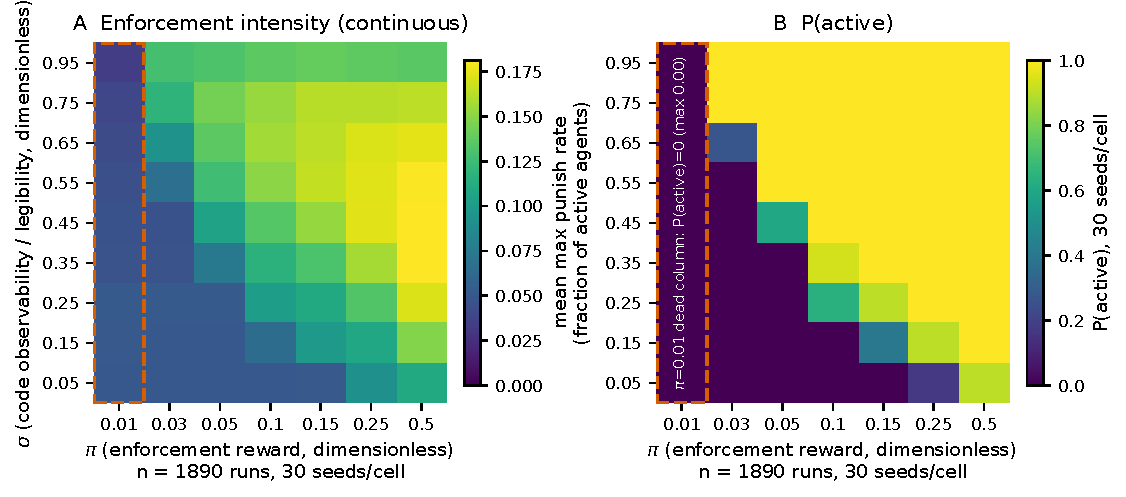
\includegraphics[width=\textwidth]{../figures/manuscript_v2/fig1_activation_frontier.pdf}
\caption{\textbf{Activation frontier under open exit.} Agent-based sweep at $\delta_0=0$ (exit open), $n=1890$ runs (9 $\sigma$ $\times$ 7 $\pi$ cells $\times$ 30 seeds per cell). (A) Mean maximum punish rate, the continuous enforcement-intensity surface. (B) Probability that a run is classified active, recomputed with the hierarchical classifier (active: max punish rate $\geq$ 0.1); overall P(active) $=$ 0.598. In the reported grid, enforcement activates only above a joint $\sigma$--$\pi$ threshold: the $\pi=0.01$ column (dashed outline) is inactive in all 9 cells, so no run in that column sustains an enforcement apparatus at any tested level of code observability.}
\label{fig:activation}
\end{figure}

\begin{figure}[htbp]
\centering
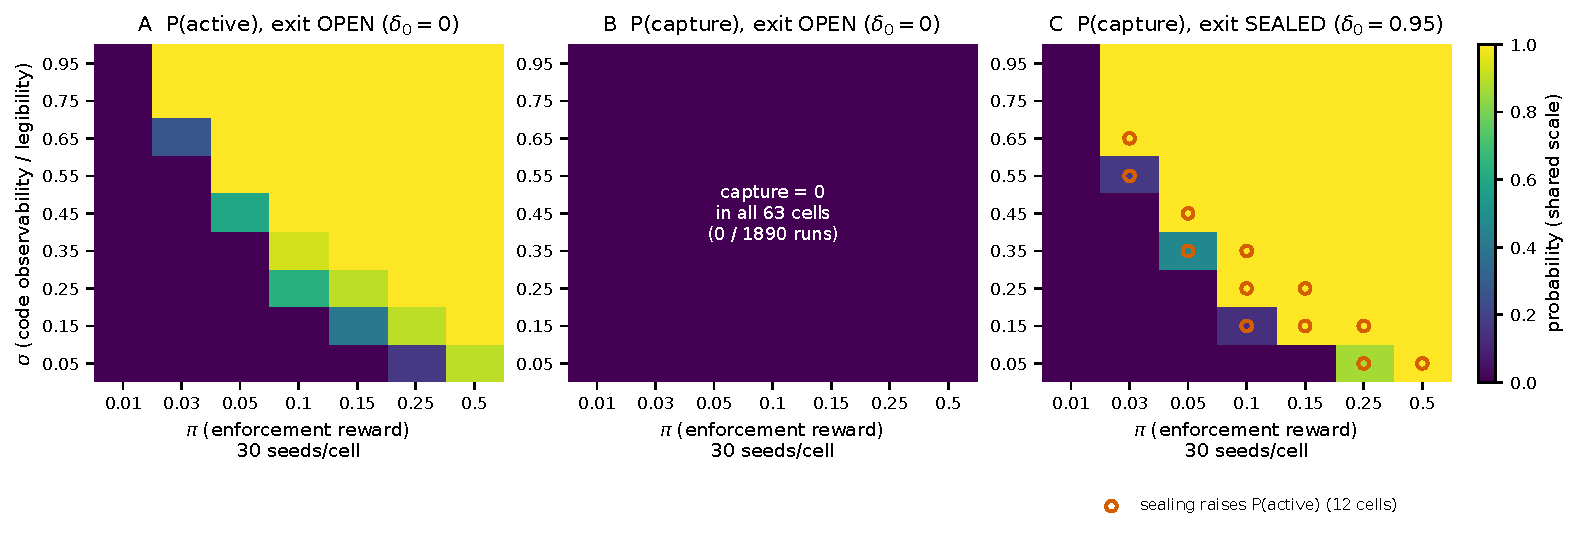
\includegraphics[width=\textwidth]{../figures/manuscript_v2/fig2_two_dimensions.pdf}
\caption{\textbf{Exit closure is necessary for capture.} All panels share one colour scale; 9 $\sigma$ $\times$ 7 $\pi$ cells $\times$ 30 seeds per cell. (A) Probability a run is active with the exit open ($\delta_0=0$, $n=1890$ runs): code geometry alone sets activation, overall P(active) $=$ 0.598. (B) Probability of capture in those same 1890 runs: \textbf{0 of 1890 runs reach capture with the exit open}; no run with the exit open reaches capture, in any of the 63 cells, despite that active rate of 0.598. (C) Probability of capture with the exit sealed ($\delta_0=0.95$, $n=1890$ runs): the active region in these runs now captures. Panels B and C are the same quantity under the two exit conditions, so the contrast isolates the effect of closing the exit. The two dimensions are not fully orthogonal: circled cells in (C) are the 12 of 63 cells where sealing also raises P(active) (mean shift over all cells +0.062; +0.328 among circled cells), and activation falls in no reported cell. Regimes recomputed with the hierarchical classifier.}
\label{fig:twodim}
\end{figure}

\begin{figure}[htbp]
\centering
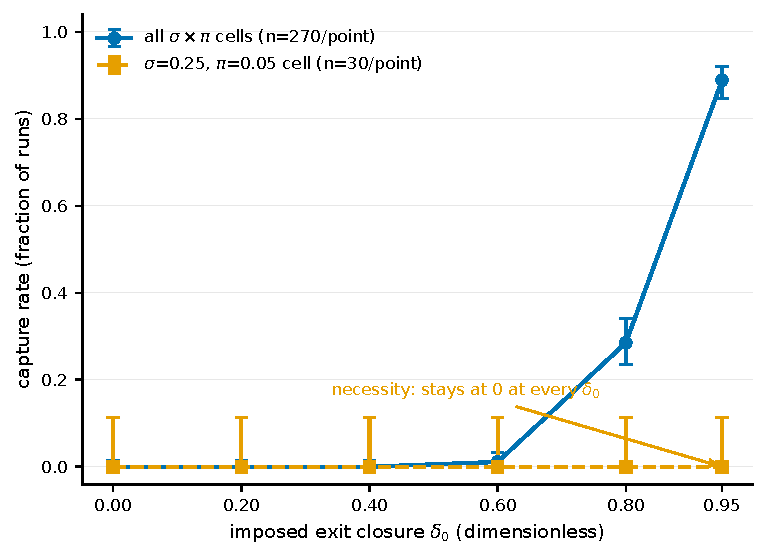
\includegraphics[width=\textwidth]{../figures/manuscript_v2/fig3_exit_closure_dose_response.pdf}
\caption{\textbf{Exit-closure dose-response and the necessity of code geometry.} Capture rate against imposed exit closure $\delta_0$ ($n=1620$ runs total; 270 runs per pooled point, 30 per cell-specific point), with Wilson 95\% intervals. Pooled over all $\sigma\times\pi$ cells (circles) capture rises monotonically from 0.000 at $\delta_0=0$ to 0.889 at $\delta_0=0.95$. In the reported runs for the $\sigma=0.25$, $\pi=0.05$ cell (squares, dashed), the capture rate is 0.000 at every tested level, including $\delta_0=0.95$: imposed closure does not produce capture in this inactive cell. Regimes recomputed with the hierarchical classifier.}
\label{fig:doseresponse}
\end{figure}

\begin{figure}[htbp]
\centering
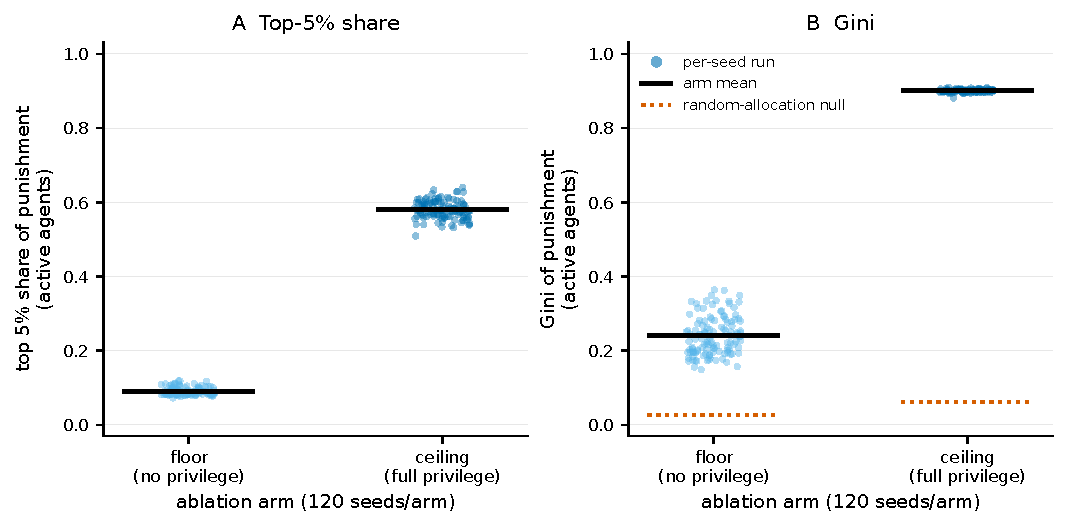
\includegraphics[width=\textwidth]{../figures/manuscript_v2/fig4_privilege_ablation.pdf}
\caption{\textbf{Concentration is manufactured by the privilege architecture.} Role-independent concentration for the ablation floor (no privilege) and ceiling (full privilege bundle), 120 seeds per arm ($n=240$ runs); points are individual runs, black bars arm means. (A) Top-5\% share of punishment among active agents rises from 0.091 at the floor to 0.580 at the ceiling, so 84\% of ceiling concentration in these runs is privilege-manufactured. (B) Gini rises from 0.240 to 0.901 against random-allocation nulls (dotted) of 0.028 and 0.062; the reported floor sits close to its null, so these runs do not show substantial concentration emerging from the unprivileged model. A committed random-allocation null exists only for the Gini statistic, so panel A carries no null reference.}
\label{fig:ablation}
\end{figure}

\begin{figure}[htbp]
\centering
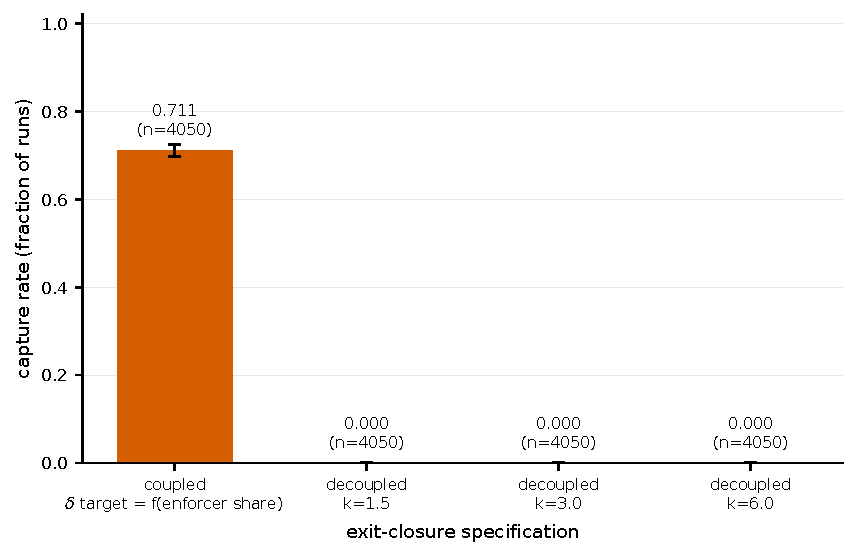
\includegraphics[width=\textwidth]{../figures/manuscript_v2/fig5_circularity_demonstration.pdf}
\caption{\textbf{Specification check for circular closure.} A specification in which outside-option closure is driven by enforcer share makes closure a function of the enforcement activity it is meant to explain ($\delta_{target} = \min(1, \delta_{baseline} + $ enforcer share$)$). Because closure enters the exit computation directly, capture then follows by construction rather than from agent behaviour; the coupled arm ($n=4050$ runs) has a capture rate of 0.711. Exit capacity is therefore treated as an independent structural input. When closure is decoupled from enforcer share and driven by punishment intensity instead, none of the tested coupling strengths produces capture: 0 of 4050 runs at each of $k=1.5$, $3.0$ and $6.0$. Wilson 95\% intervals are shown; regimes are computed with the hierarchical classifier, under which capture is retained AND active and enforcer share is not itself a criterion.}
\label{fig:circularity}
\end{figure}

\section*{Acknowledgments}

% ============================================================
% REFERENCES
% ============================================================

% ============================================================
% Bibliography.
% The canonical bibliographic data live in references.bib. This
% thebibliography block is generated from that file in author-year
% form, sorted alphabetically, because bibtex is not available in
% the build environment. With bibtex present, delete the block
% below and uncomment the following line; \bibliographystyle{plainnat}
% is already set in the preamble.
%\bibliography{references}
% ============================================================
\begin{thebibliography}{43}

\bibitem[Axelrod(1986)]{axelrod1986}
Axelrod R (1986) An evolutionary approach to norms. \textit{American Political Science Review} 80(4):1095--1111.

\bibitem[Berman(2000)]{berman2000}
Berman E (2000) Sect, subsidy, and sacrifice: An economist's view of ultra-Orthodox Jews. \textit{Quarterly Journal of Economics} 115(3):905--953.

\bibitem[Berman and Laitin(2008)]{bermanlaitin2008}
Berman E, Laitin DD (2008) Religion, Terrorism and Public Goods: Testing the Club Model. \textit{Journal of Public Economics} 92(10--11):1942--1967.

\bibitem[Berman and Laitin(2008)]{berman2008}
Berman E, Laitin DD (2008) Religion, terrorism and public goods: Testing the club model. \textit{Journal of Public Economics} 92(10--11):1942--1967.

\bibitem[Bok(2025)]{bok2025}
Bok J (2025) Religious Exit Costs. \textit{Journal for the Scientific Study of Religion} 64(2):227--239. doi:10.1111/jssr.12963.

\bibitem[Boyd et~al.(2010)]{boydgintisbowles2010}
Boyd R, Gintis H, Bowles S (2010) Coordinated Punishment of Defectors Sustains Cooperation and Can Proliferate When Rare. \textit{Science} 328(5978):617--620. doi:10.1126/science.1183665.

\bibitem[Boyd et~al.(2003)]{boyd2003}
Boyd R, Gintis H, Bowles S, Richerson PJ (2003) The evolution of altruistic punishment. \textit{Proceedings of the National Academy of Sciences} 100(6):3531--3535.

\bibitem[Bromley(1998)]{bromley1998}
Bromley DG (1998) The Politics of Religious Apostasy: The Role of Apostates in the Transformation of Religious Movements. Praeger.

\bibitem[Carvalho(2013)]{carvalho2013}
Carvalho JP (2013) Veiling. \textit{Quarterly Journal of Economics} 128(1):337--370.

\bibitem[Carvalho(2019)]{carvalho2019}
Carvalho JP (2019) Religious Clubs: The Strategic Role of Religious Identity. In: Carvalho JP, Iyer S, Rubin J (eds) \textit{Advances in the Economics of Religion}, International Economic Association Series, vol 158. Palgrave Macmillan, Cham, pp 25--41.

\bibitem[Centola et~al.(2005)]{centola2005}
Centola D, Willer R, Latan\'e B (2005) The emperor's dilemma: A computational model of self-enforcing norms. \textit{American Journal of Sociology} 110(4):1009--1040.

\bibitem[Cook(2000)]{cook2000}
Cook M (2000) Commanding Right and Forbidding Wrong in Islamic Thought. Cambridge University Press.

\bibitem[Cragun and Hammer(2011)]{cragun2011}
Cragun RT, Hammer JH (2011) One person's apostate is another person's convert: What terminology tells us about pro-religious hegemony in the sociology of religion. \textit{Humanity \& Society} 35(1--2):149--175.

\bibitem[Fehr and G\"achter(2000)]{fehr2000}
Fehr E, G\"achter S (2000) Cooperation and punishment in public goods experiments. \textit{American Economic Review} 90(4):980--994.

\bibitem[Fehr and G\"achter(2002)]{fehr2002}
Fehr E, G\"achter S (2002) Altruistic punishment in humans. \textit{Nature} 415(6868):137--140.

\bibitem[Fehr and G\"{a}chter(2000)]{fehrgachter2000}
Fehr E, G\"{a}chter S (2000) Cooperation and Punishment in Public Goods Experiments. \textit{American Economic Review} 90(4):980--994. doi:10.1257/aer.90.4.980.

\bibitem[Gelfand et~al.(2011)]{gelfand2011}
Gelfand MJ, et al (2011) Differences between tight and loose cultures: A 33-nation study. \textit{Science} 332(6033):1100--1104.

\bibitem[Given(1997)]{given1997}
Given JB (1997) Inquisition and Medieval Society: Power, Discipline, and Resistance in Languedoc. Cornell University Press.

\bibitem[Gore et~al.(2018)]{gorelemosshultswildman2018}
Gore R, Lemos C, Shults FL, Wildman WJ (2018) Forecasting Changes in Religiosity and Existential Security with an Agent-Based Model. \textit{Journal of Artificial Societies and Social Simulation} 21(1):4. doi:10.18564/jasss.3596.

\bibitem[Greif(2006)]{greif2006}
Greif A (2006) Institutions and the Path to the Modern Economy: Lessons from Medieval Trade. Cambridge University Press.

\bibitem[Greif and Mokyr(2016)]{greif2016}
Greif A, Mokyr J (2016) Cognitive rules, institutions, and economic growth: Douglass North and beyond. \textit{Journal of Institutional Economics} 13(1):25--52.

\bibitem[Hauert et~al.(2007)]{hauertetal2007}
Hauert C, Traulsen A, Brandt H, Nowak MA, Sigmund K (2007) Via Freedom to Coercion: The Emergence of Costly Punishment. \textit{Science} 316(5833):1905--1907.

\bibitem[Hilbe et~al.(2014)]{hilbe2014}
Hilbe C, Traulsen A, R\"ohl T, Milinski M (2014) Democratic decisions establish stable authorities that overcome the paradox of second-order punishment. \textit{Proceedings of the National Academy of Sciences} 111(2):752--756.

\bibitem[Hirschman(1970)]{hirschman1970}
Hirschman AO (1970) Exit, Voice, and Loyalty: Responses to Decline in Firms, Organizations, and States. Harvard University Press.

\bibitem[Iannaccone(1988)]{iannaccone1988}
Iannaccone LR (1988) A Formal Model of Church and Sect. \textit{American Journal of Sociology} 94(Supplement):S241--S268. doi:10.1086/228948.

\bibitem[Iannaccone(1992)]{iannaccone1992}
Iannaccone LR (1992) Sacrifice and Stigma: Reducing Free-Riding in Cults, Communes, and Other Collectives. \textit{Journal of Political Economy} 100(2):271--291.

\bibitem[Iannaccone(1994)]{iannaccone1994}
Iannaccone LR (1994) Why Strict Churches Are Strong. \textit{American Journal of Sociology} 99(5):1180--1211.

\bibitem[Iannaccone and Makowsky(2007)]{iannacconemakowsky2007}
Iannaccone LR, Makowsky MD (2007) Accidental Atheists? Agent-Based Explanations for the Persistence of Religious Regionalism. \textit{Journal for the Scientific Study of Religion} 46(1):1--16.

\bibitem[Iyer(2016)]{iyer2016}
Iyer S (2016) The New Economics of Religion. \textit{Journal of Economic Literature} 54(2):395--441. doi:10.1257/jel.54.2.395.

\bibitem[Kelly(1989)]{kelly1989}
Kelly HA (1989) Inquisition and the prosecution of heresy: Misconceptions and abuses. \textit{Church History} 58(4):439--451.

\bibitem[Kuran(1995)]{kuran1995}
Kuran T (1995) Private Truths, Public Lies: The Social Consequences of Preference Falsification. Harvard University Press.

\bibitem[Mann(1986)]{mann1986}
Mann M (1986) The Sources of Social Power, Vol. 1. Cambridge University Press.

\bibitem[McBride(2007)]{mcbride2007}
McBride M (2007) Club Mormon: Free-Riders, Monitoring, and Exclusion in the LDS Church. \textit{Rationality and Society} 19(4):395--424. doi:10.1177/1043463107083736.

\bibitem[Norenzayan and Gervais(2013)]{norenzayan2013}
Norenzayan A, Gervais WM (2013) The origins of religious disbelief. \textit{Trends in Cognitive Sciences} 17(1):20--25.

\bibitem[North(1990)]{north1990}
North DC (1990) Institutions, Institutional Change and Economic Performance. Cambridge University Press.

\bibitem[Pierson(2000)]{pierson2000}
Pierson P (2000) Increasing returns, path dependence, and the study of politics. \textit{American Political Science Review} 94(2):251--267.

\bibitem[Rubin(2017)]{rubin2017}
Rubin J (2017) Rulers, Religion, and Riches: Why the West Got Rich and the Middle East Did Not. Cambridge University Press.

\bibitem[Scott(1998)]{scott1998}
Scott JC (1998) Seeing Like a State: How Certain Schemes to Improve the Human Condition Have Failed. Yale University Press.

\bibitem[Sigmund et~al.(2010)]{sigmund2010}
Sigmund K, De Silva H, Traulsen A, Hauert C (2010) Social learning promotes institutions for governing the commons. \textit{Nature} 466(7308):861--863.

\bibitem[Streib et~al.(2009)]{streib2009}
Streib H, Hood RW, Keller B, Cs\"off RM, Silver CF (2009) Deconversion: Qualitative and Quantitative Results from Cross-Cultural Research in Germany and the United States of America. Vandenhoeck \& Ruprecht.

\bibitem[Tilly(1985)]{tilly1985}
Tilly C (1985) War making and state making as organized crime. In: Evans P, Rueschemeyer D, Skocpol T (eds) \textit{Bringing the State Back In}. Cambridge University Press, pp 169--191.

\bibitem[Weber(1946)]{weber1946}
Weber M (1946) Politics as a Vocation. In: Gerth HH, Mills CW (eds) \textit{From Max Weber: Essays in Sociology}. Oxford University Press, pp 77--128. (Original work published 1919.)

\bibitem[Wildman and Sosis(2011)]{wildmansosis2011}
Wildman WJ, Sosis R (2011) Stability of Groups with Costly Beliefs and Practices. \textit{Journal of Artificial Societies and Social Simulation} 14(3):6. doi:10.18564/jasss.1781.

\end{thebibliography}

\section*{Data and Code Availability}

All simulation code, data, and analysis scripts are publicly available: an anonymized review copy of the repository is available at [ANONYMOUS-LINK]; the public archive will be linked upon acceptance.

\section*{Supporting Information}

\noindent\textbf{Online Resource 1.} Scoring rubric anchors (0--4 scale definitions for all five code-geometry dimensions), complete parameter tables, illustrative regime scores with source citations, regime classification threshold sensitivity ($\pm$5 pp), monopoly ablation results (180 runs), and cadre quota sensitivity (180 runs).

\end{document}
